\documentclass[tikz]{standalone}

\usetikzlibrary{shapes,arrows,shadows,calc, angles}
\usetikzlibrary{arrows,shapes}
\usetikzlibrary{positioning}
\usetikzlibrary{patterns.meta}

\usetikzlibrary{decorations, decorations.pathreplacing}

\definecolor{fg}{rgb}{0,0,0}
\definecolor{bg}{rgb}{1,1,1}

\tikzstyle{box}=[draw, rounded corners, thick,
anchor=center,text centered,text=fg, font=\bfseries] % text width=33mm,

\tikzstyle{myarrow}=[->, >=stealth, thick, rounded corners=2mm]
\tikzstyle{mythinarrow}=[myarrow, line width=0.25mm]

\begin{document}

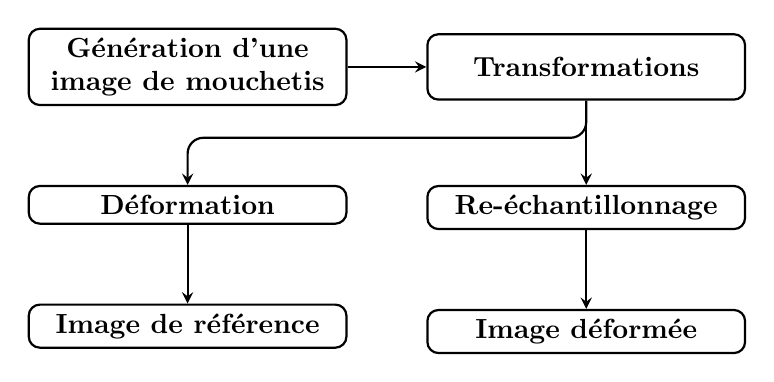
\begin{tikzpicture}
    \node (A0) at (0, 0) {} ;
    \node (B0) at (40mm, 0) {} ;
    \node (Ca0) at (0, -20mm) {} ;
    \node (Cb0) at (40mm, -20mm) {} ;

    \node[box, text width=38mm] (A) {Génération d'une image de mouchetis};
    \node[box, text width=38mm, minimum height=8.3mm, right=of A] (B)
        {Transformations} ;
    \node[box, text width=38mm, below=of A] (Ca) {Déformation} ;
    \node[box, text width=38mm, below right=of A] (Cb) {Re-échantillonnage} ;
    \node[box, text width=38mm, below=of Ca] (Da) {Image de référence} ;
    \node[box, text width=38mm, below=of Cb] (Db) {Image déformée} ;

    \draw[myarrow] (A) -- (B) ;
    \draw[myarrow] (B) -- ++ (0, -9mm) -| (Ca) ;
    \draw[myarrow] (B) -- (Cb) ;
    \draw[myarrow] (Ca) -- (Da) ;
    \draw[myarrow] (Cb) -- (Db) ;
\end{tikzpicture}

\end{document}